In this section, we initiate a comprehensive analysis to reveal the stability of established tool benchmarks, using Toolbench~\citep{qin2023tool} as a case study.
We examine the stability of ToolBench by investigating three key dimensions: performance, evaluation, and API status.

\subsection{Stability of Performance}\label{sec:pre_analysis_performance}

Benchmarks are designed to consistently evaluate the performance of various models over time.
To test this consistency, we reproduce the model performances and record any variations.
Our study employs Chain-of-Thought (CoT;~\citealp{wei2023chainofthought}) and Depth First Search (DFS) strategies, leveraging ChatGPT and ToolLLaMA for comparative analysis.
We adhere strictly to the configurations detailed in ToolBench, utilising the ChatGPT version \texttt{gpt-3.5-turbo-0613} and \texttt{ToolLLaMA-v2}.
As depicted in \Cref{fig:performance_comparison_failure}, we compare the original Pass Rates for the I1-Instruction group reported by ToolBench with the Pass Rates we reproduced for four conventional methods.
\begin{figure}[]
    \centering
    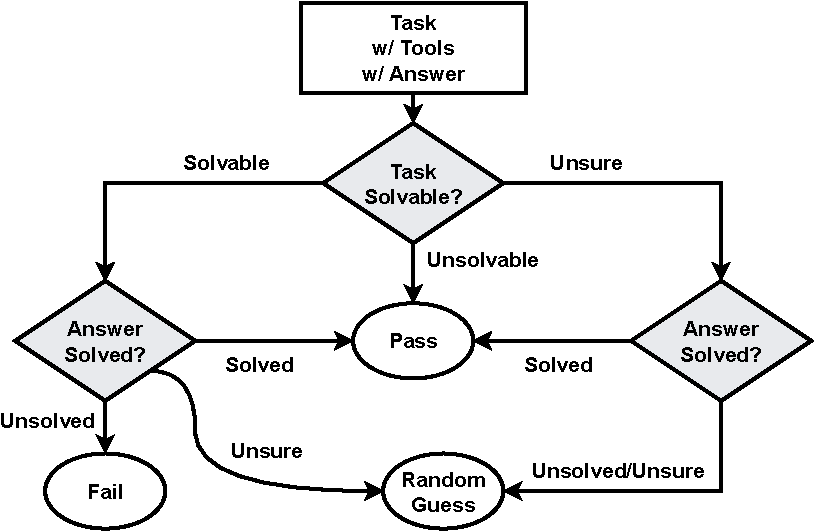
\includegraphics[width=\linewidth]{figs/PR.pdf}
    \caption{Pass Rate evaluation in ToolBench paper.}
    \label{fig:pass-rate}
\end{figure}
Our findings indicate a notable decline in the performance of all methods over time, which raises concerns about the stability of ToolBench as a benchmark.



% \begin{figure*}
%     % \centering
%     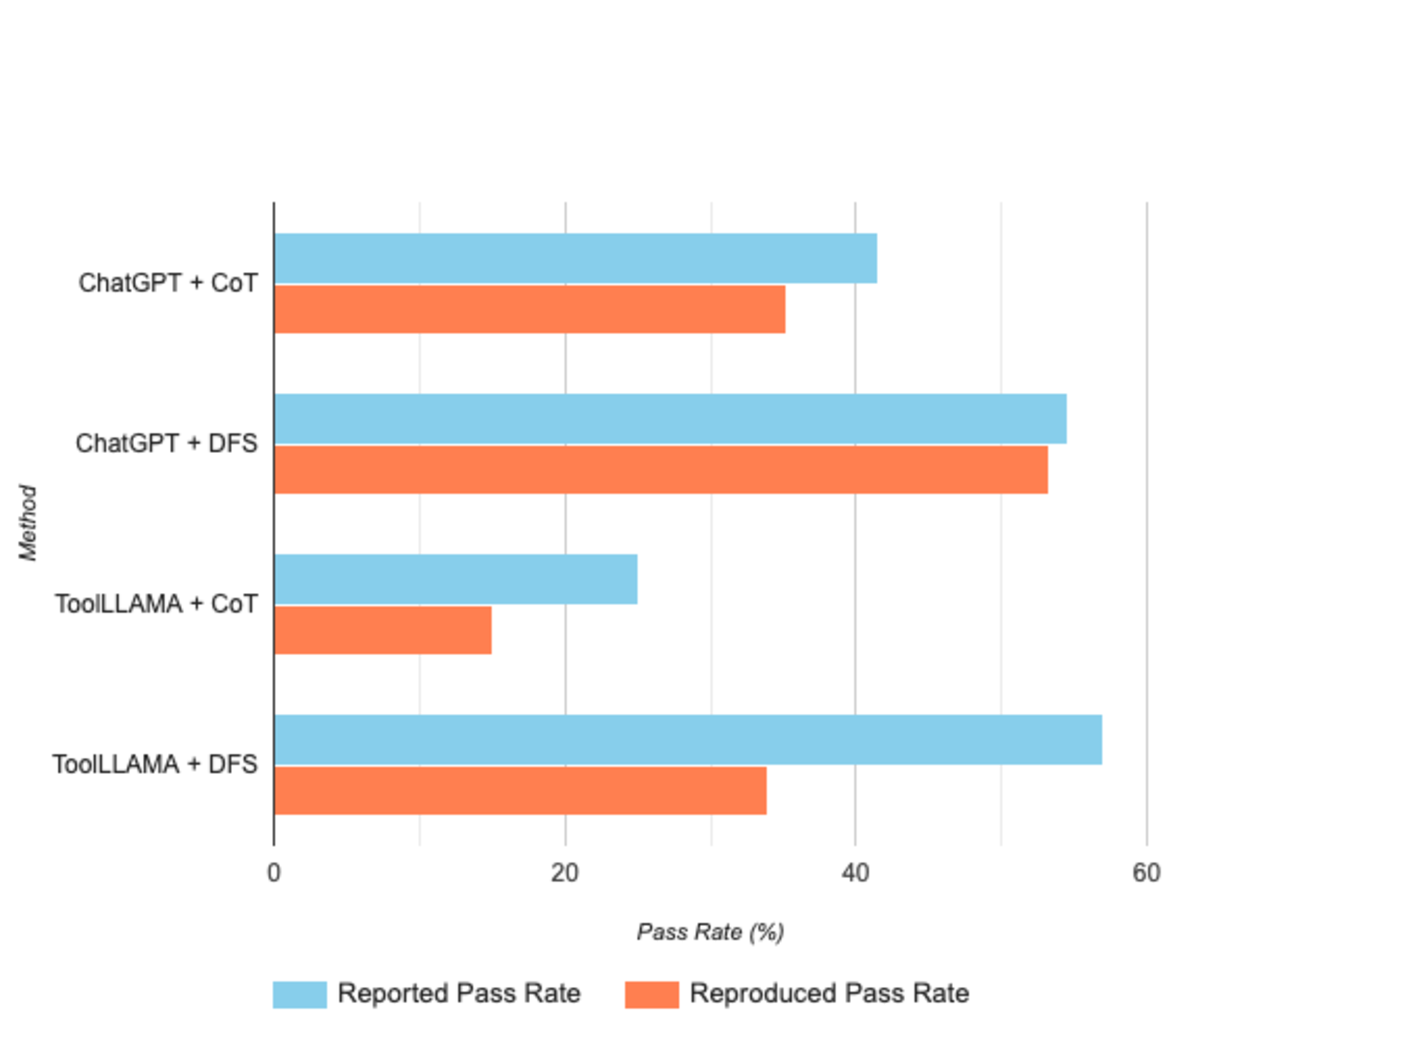
\includegraphics[width=\textwidth]{figs/table_2_perf_comparison.pdf} 
%     \caption{Comparison of performance (Pass Rate) reported in the paper and reproduced by us of ChatGPT and ToolLLaMA v2 on the I1-Instruction group of ToolBench.}
%     \label{tab:performance_comparison}
% \end{figure*}


\subsection{Stability of Evaluation}
\label{sta_eval}

In ToolBench, there are two types of metrics, including Pass Rate (PR) and Win Rate (WR). 
% PR is automatically evaluated by \texttt{gpt-3.5-turbo-16k}.
PR is calculated based on using \texttt{gpt-3.5-turbo-16k} to determine if a task is solvable and whether the generated answer can solve the corresponding task.
% PR is then calculated based on the solvability of the task and the effectiveness of the answer.
% The statuses of tasks are categorized as solvable, unsolvable, or unsure, while the statuses of answers can be solved, unsolved, or unsure.
\Cref{fig:pass-rate} details the computation process of PR.
Specifically, a solvable task results in a pass if the answer is solved, a failure if unsolved, and is randomly determined if unsure.
For tasks deemed unsure, a pass is assigned only if the answer is solved; otherwise, a random outcome is chosen.
If a task is unsolvable, the result defaults to a pass regardless of the answer status.
Moreover, WR is derived from the comparative PR of paired candidates.
% as shown in~\Cref{todo}.
A candidate's WR increases by one each time it passes while the other fails.
In all other situations, WR relies on \texttt{gpt-3.5-turbo-16k} to automatically evaluate the paired candidates.

% Please add the following required packages to your document preamble:
% \usepackage{multirow}
% Please add the following required packages to your document preamble:
% \usepackage{multirow}
% \begin{table}[]
% \small
% \centering
% \begin{tabular}{l|l|l|c|l}
% \toprule
%  & \multicolumn{3}{c}{\textbf{Task Status}} \\
%  & Solvable & \multicolumn{1}{l}{Unsolvable} & Unsure \\
%  \cmidrule
% Solved & Passed & \multirow{3}{*}{Passed} & Passed \\
% Unsolved & Failed &  & \multirow{2}{*}{Random} \\
% Unsure & Random &  &\\
% \bottomrule
% \end{tabular}
% \end{table}



\begin{table}[t!]
    \small
    \centering
    \resizebox{\linewidth}{!}{
    \begin{tabular}{l|ccc|ccc|c|c}
    \toprule
    \multirow{2}{*}{\textbf{Method}} & \multicolumn{3}{c|}{\textbf{Task}} & \multicolumn{3}{c|}{\textbf{Answer}} & \multirow{2}{*}{\textbf{Pass}} & \multirow{2}{*}{\textbf{Win}} \\
    & S & US & UE & S & US & UE & & \\
    \midrule
        \multirow{3}{*}{CoT} & 168 & 23 & 9 & 19 & 170 & 11 & 33.0 & 50.0 \\
         & 165 & 29 & 6 & 16 & 174 & 10 & 31.5 & 46.5 \\
         & 151 & 40 & 9 & 20 & 167 & 13 & 37.5 & 53.0 \\
        \midrule
        \multirow{3}{*}{DFS} & 116 & 68 & 16 & 17 & 167 & 16 & 50.5 & 54.0 \\
         & 122 & 59 & 19 & 20 & 162 & 18 & 46.5 & 48.0 \\
         & 132 & 54 & 14 & 22 & 157 & 21 & 55.0 & 56.0 \\
    \bottomrule
    \end{tabular}}
    \caption{Experiments use \texttt{GPT-3.5-Turbo-0613} with CoT and DFS. S, US, and UE indicate solvable (solved), unsolvable (unsolved), and unsure. Pass and Win denote pass rate and win rate, respectively. Win rates are evaluated against the first run of CoT. This experiment is run on 4 Feb 2024.}
    \label{tab:sta_eval}
\end{table}

To assess the stability of evaluation, we perform both CoT and DFS using \texttt{gpt-3.5-turbo-0613} on the I1-Instruction group dataset. 
These analyses are conducted using the provided tools and repeat over three iterations each.
The resulting PR and WR are presented in~\Cref{tab:sta_eval}, with detailed task and answer items.
% Although DFS generally exhibits higher PR than CoT, the distribution of tasks and answers is illogical.
Despite PRs of DFS being generally higher than CoT, the contribution of the task is larger than the answer.
However, it is worth noting that the tasks are the same in both CoT and DFS, where their results are expected to be consistent.
On the contrary, the discrimination of answers between CoT and DFS is weak, where a considerable proportion are unsolved.
Moreover, WR does not reflect the same trend as PR, where the second run of WR in DFS (48.0) is even lower than the first run of CoT.
Therefore, all the phenomena reflect that \texttt{gpt-3.5-turbo-16k} can not assume the role of the automatic evaluator in tool learning, which will be discussed in~\Cref{sec:evaluator}.


% \begin{figure}[h!]
%     \centering  
%      \begin{subfigure}[b]{\linewidth}
%         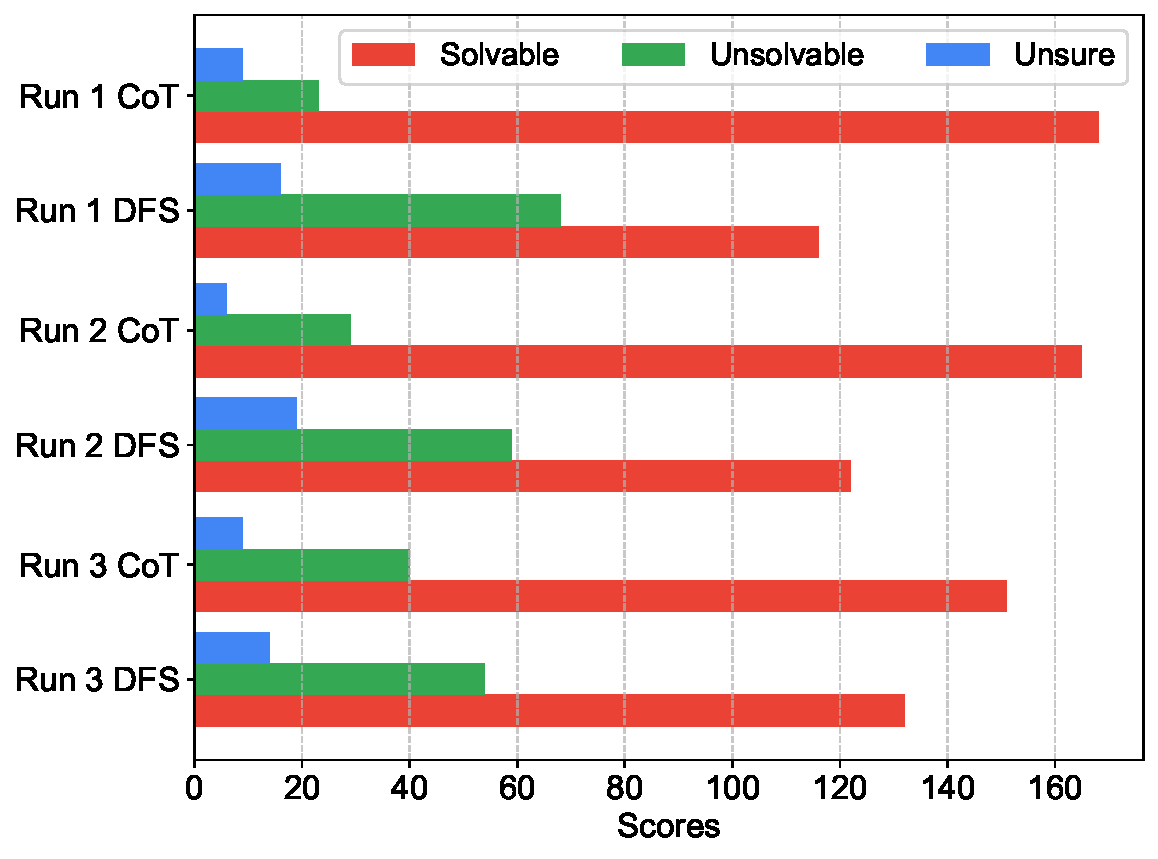
\includegraphics[width=\linewidth]{figs/task_status_count.pdf}
%         \caption{Task Status}
%       \end{subfigure}
%       \begin{subfigure}[b]{\linewidth}
%     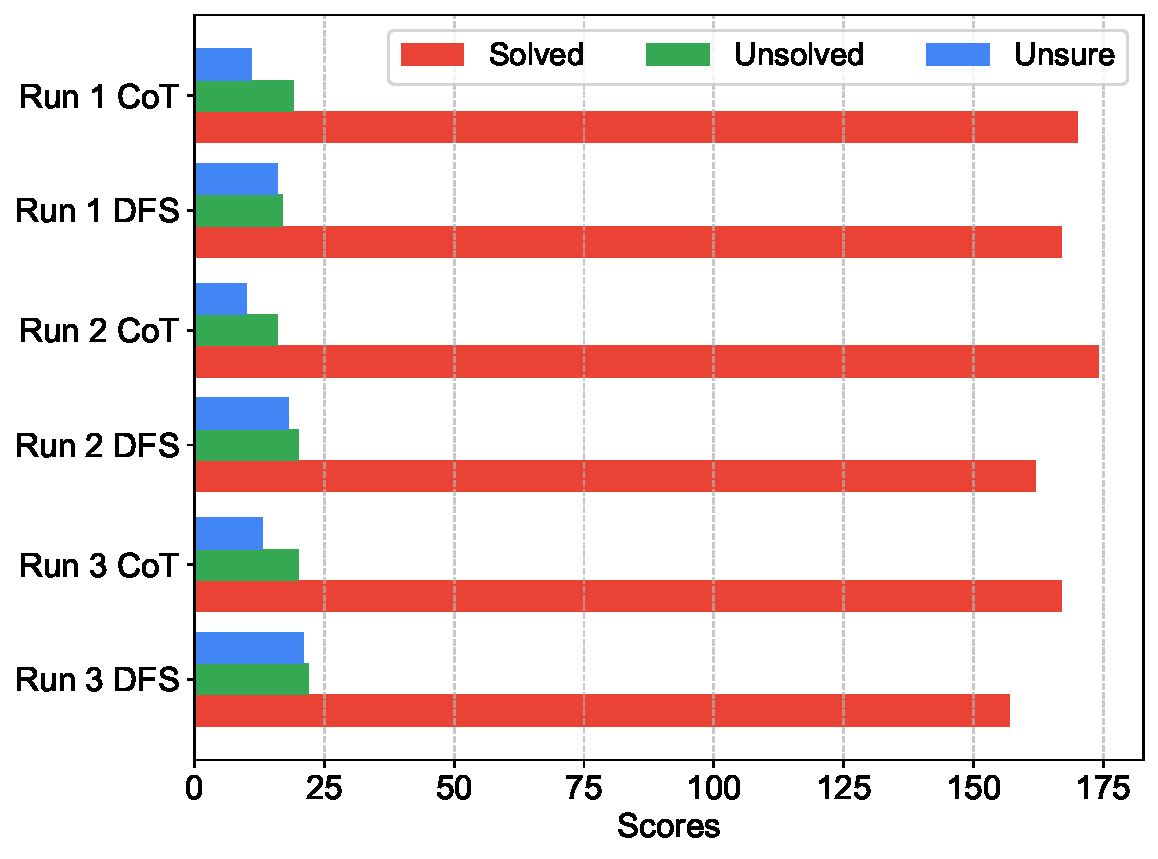
\includegraphics[width=\linewidth]{figs/answer_status_count.pdf}
%     \caption{Answer Status}
%       \end{subfigure}
    
%     \caption{Task and Answer status}
%     \label{fig:sta_eval}
% \end{figure}

% \begin{figure}[ht!]
%     \centering
%     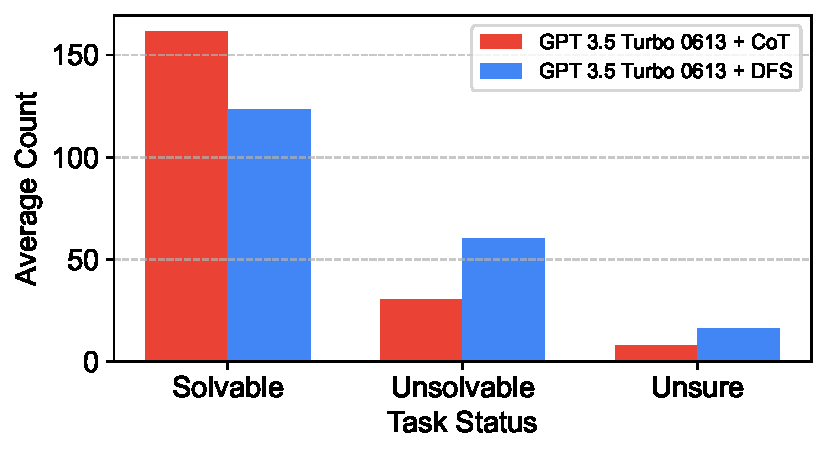
\includegraphics[width=\linewidth]{figs/status_eval.pdf}
%     \caption{Task and Answer status}
%     \label{fig:sta_eval}
% \end{figure}




\subsection{Stability of API Status}
\label{api_status}
% \textcolor{red}{Discuss the phenomenon that APIs are not callable in ToolBench and ToolEyes. These are resulting from authentication, documentation change, etc}.
% Results shown in \Cref{fig:toolbench-api-status}.
% To find the causes of the aforementioned instability,
We investigate the change of API status in ToolBench. 
In detail, we scan the original APIs downloaded from ToolBench, and use \texttt{gpt-4-turbo} to automatically write calls via the prompts as shown in \Cref{app:prompt_make_call}.
According to the keyword in API feedback, we classify these APIs into three categories: success, not availability, and not authorisation\footnote{Note that we use the \texttt{toolbench-key} provided in ToolBench to simulate the real running process in the benchmark.}.
The API status and the detailed errors of not availability are presented in \Cref{fig:api_change_info}. 
\begin{figure}[]
    \centering   
    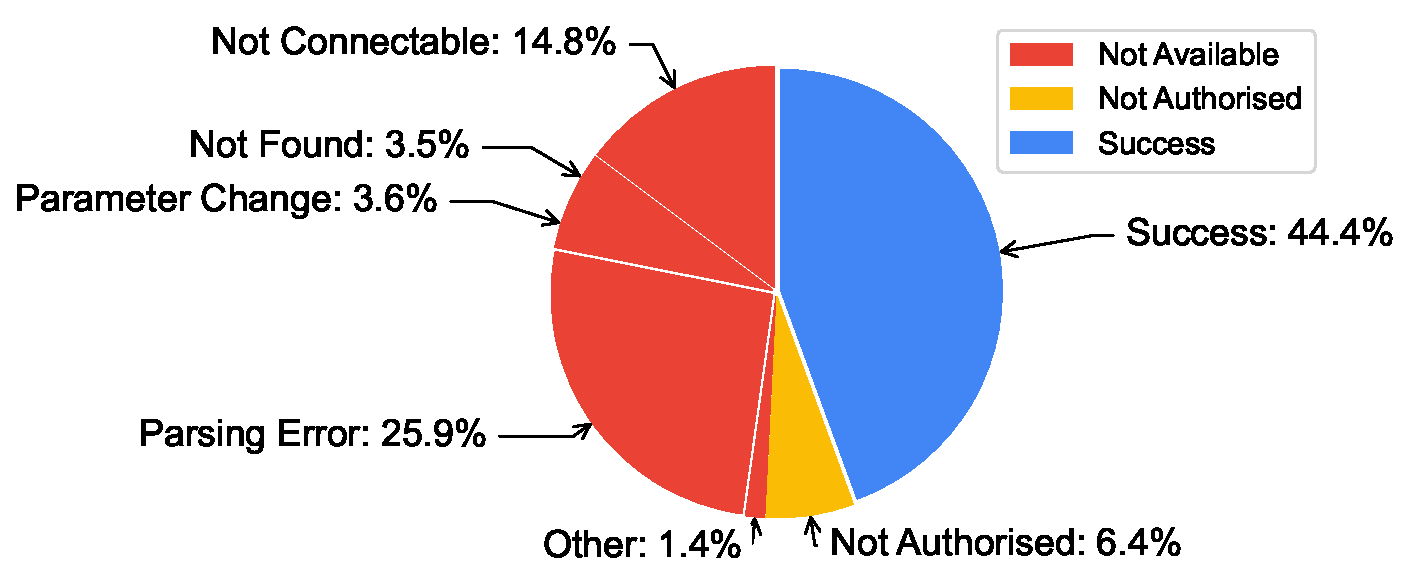
\includegraphics[width=\linewidth]{figs/api_status_merged.pdf}
    \caption{Statistics of API changes. Parsing errors are caused by post-processing errors of local API documentation, which have been solved in our benchmark.}
   
    \label{fig:api_change_info}
\end{figure}
As can be seen, only 44.4\% of API calls are successful, while other API calls are mostly not available with various errors and some are not authorised.

% As for the not available APIs, xxx.

% authentication: 1058
% request_failure: 2426
% parameter: 591
% not_working: 248
% not_found: 583
% bugs: 4247




% \begin{table}[h!]
%     \centering
%     \small
%     \begin{tabular}{cc}
%      \toprule
%     \textbf{Status Type} & \textbf{Percentage} (\%) \\
%     \midrule
%     % No Change & 83.3 \\
%     % Parameter Change & 16.7 \\
%         No Change & 84.5 \\
%     Parameter Change & 15.5 \\
%      \bottomrule
%     \end{tabular}
%     \caption{APIs changed in ToolBench.}
%     \label{tab:api_change}
% \end{table}
\begin{figure}[h!]
    \centering
    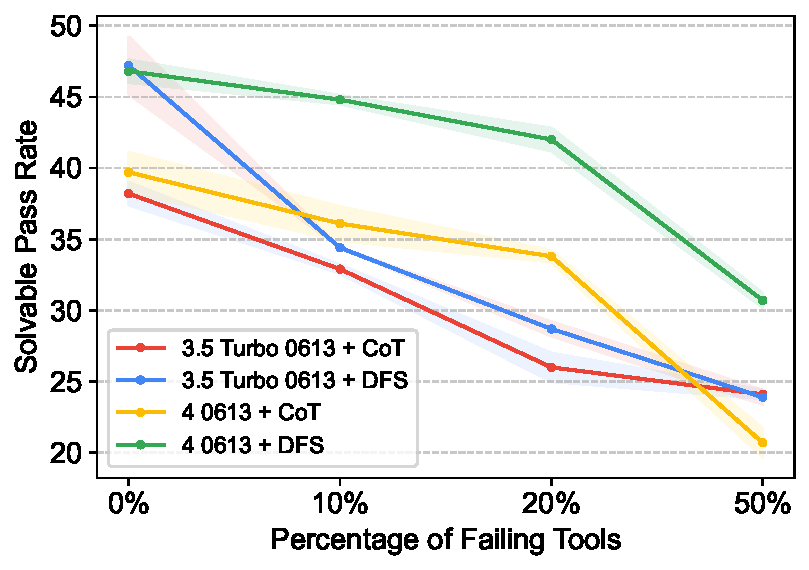
\includegraphics[width=\linewidth]{figs/real_solving_scores.pdf}
    \caption{Solvable Pass Rate (SoPR) change when manually making APIs down on the I1 Instruction group.}
    \label{fig:real_api_stability_test}
\end{figure}


\begin{figure*}[t!]
    \centering
    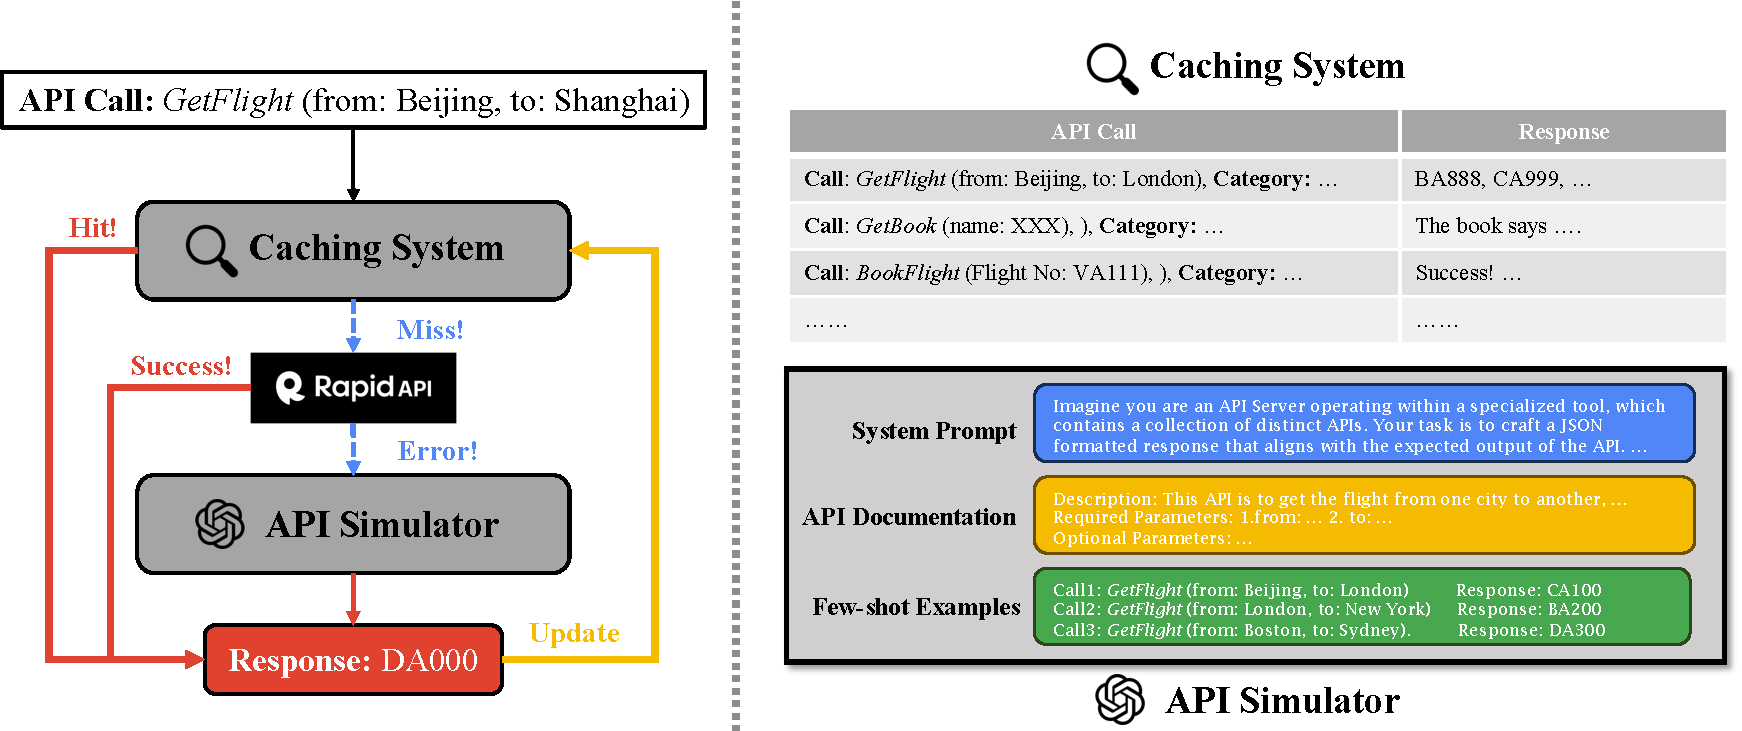
\includegraphics[width=\textwidth]{figs/main_figure.pdf} 
    \caption{The process of calling APIs in our proposed virtual API server.}
    \label{fig:main_figure}
\end{figure*}


% \begin{figure}[h!]
%     \centering
%     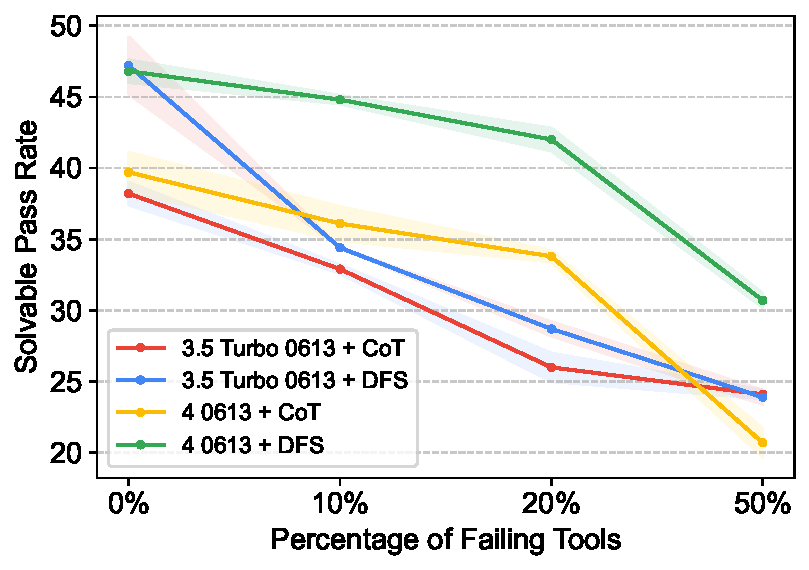
\includegraphics[width=\linewidth]{figs/real_solving_scores.pdf}
%     \caption{Solvable Pass Rate (SoPR) change when manually making APIs down on the I1 Instruction group.}
%     \label{fig:real_api_stability_test}
% \end{figure}
Furthermore, to validate the impact of API call failures on the stability of model performance, we manually make some success tools\footnote{In ToolBench, a tool is composed of several APIs. For example, a database tool can have two APIs: a writing API and a reading API. } down by returning a special failure call. Specifically, we randomly sample a proportion of success tools containing success APIs found in \Cref{fig:api_change_info}.
At testing time, when sampled tools are called, a special response will be thrown: \texttt{\{``error'': ``'', ``response'': ``This API did not return any useful information...''\}} to simulate the API call failures. 
We conduct baseline models with different proportions (i.e., 0\%, 10\%, 20\%, and 50\%) of sampled APIs on the I1 Instruction set.
% To confirm that the sampled tools will be called, we calculate the proportions of ground truth tools appearing in the sampled tools. 
% The results are shown in \Cref{app:proportion_sampling}.
Due to the issues in evaluation, we use our stable evaluation system proposed in~\Cref{sec:evaluation_system} as the same as our main experiments.
For each experiment, we evaluate three times and report the average scores as shown in \Cref{fig:real_api_stability_test}.
It can be seen that the performance degrades a lot when the proportion of successful APIs is down, thus the impact of API status on stability is considerable.

% \begin{figure}[h!]
%     \centering
%     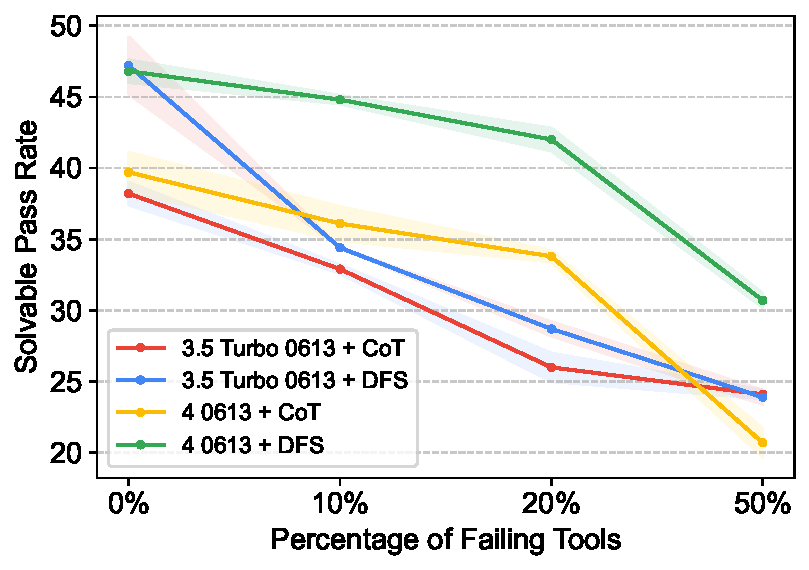
\includegraphics[width=\linewidth]{figs/real_solving_scores.pdf}
%     \caption{Solvable Pass Rate (SoPR) change when manually making APIs down on the I1 Instruction group.}
%     \label{fig:real_api_stability_test}
% \end{figure}

% \subsection{Stability of API Document}

% It is worth noting that we can only simulate functions calling varying very small parts of parameters, thus there may be other parameter errors.
% Therefore, secondly, we directly investigate into the parameter changes in all API documentation over time.
% % sample 50 APIs used in ToolBench and 
% We crawl the current document corresponding to the API in Toolbench from RapidAPI\footnote{\url{https://rapidapi.com}}. 
% Then, we check whether the parameter information of these APIs is changed and the results on parameter changes are shown in \Cref{tab:api_change}. It shows that a significant portion (16.7\%) of APIs change their documentation, which may affect the stability of model performance.

% \begin{figure}
%     \centering
%     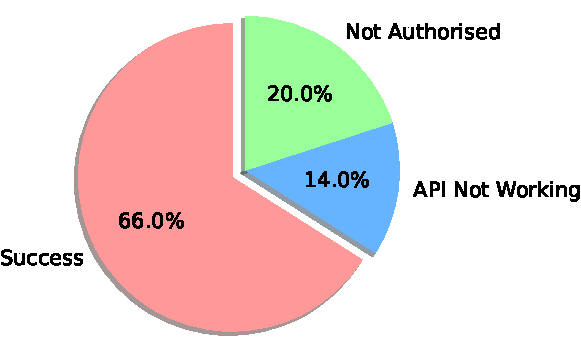
\includegraphics[width=\linewidth]{figs/toolbench_api_statistics.pdf}
%     \caption{API status in ToolBench. We sample 50 APIs in the APIs used in ToolBench and manually label the status of these APIs.}
%     \label{fig:toolbench-api-status}
% \end{figure}

% We manually let some APIs down to test the impact of API stability on model performance. [Experimental Setups] Results are shown in \Cref{tab:real_api_stability_test}.[Results analysis] 



% \begin{table}[]
%     \centering
%     \small
%     \begin{tabular}{cccc}
%         \toprule
%         \multirow{2}{*}{\textbf{Method}} & \multicolumn{3}{c}{\textbf{Percentage of Failing APIs}}\\
%         % \cmidrule{2-5}
%           & 10\% & 20\% & 50\% \\
%         \midrule
%          ChatGPT + CoT & 47.5 & 49.5 & 32.5 \\
%          ChatGPT + DFS & 47.0 & 46.0 & 34.5  \\
%          ToolLLaMA + CoT & 48.0 & 47.0 \\
%          ToolLLaMA + DFS & 50.5 & 50.5 \\
%          \bottomrule
%     \end{tabular}
%     \caption{Win rate against no change when manually make APIs down on the I1 Instruction group.}
%     \label{tab:real_api_stability_test}
% \end{table}
